\cotefile{74}
\scanpage{73}

% top, lines 1–2
\[
\begin{aligned}
\unsure{120|720}\quad\mathrm{Hex}&=\text{ens des hexagones de trièdres \inserted{liées (de $\Delta$)} ( ``grands hexagones'')}\\
&\simeq\text{ens des pavés}
\end{aligned}
\]

% top, lines 3–4
\[
\begin{aligned}
720\quad\mathrm{hex}&=\text{ens des hexagones de sommets \inserted{de $\Delta$} \deleted{\unsure{$\Delta$}} (= ``petits hex.'')}\\
21\quad &\simeq\text{ens des paires de trièdres opposables}
\end{aligned}
\]

% top, lines 5–6
\[
\begin{aligned}
&\deleted{\simeq\text{ens des couples }(X,t),\ X\text{ pavé et }t\in X}\\
720\quad\mathrm{tria}&=\deleted{\text{ens des \unsure{trièdres|triades}}}
\end{aligned}
\]

% upper, lines 7–8
\[
40\quad\mathrm{triHex}\simeq\text{ens des triples (non ordonnés) \inserted{``distingués''} de grands hexagones,\,/ i.e.}
\]

% upper, lines 9–10
\[
\begin{aligned}
360\quad(\mathrm{tria}')&\simeq\text{ens des \inserted{paires de} trièdres \inserted{opposés} \deleted{\unsure{(liés) = ens des pai|(Tria' = ens des pai}}}\\
&\hspace{2em}\text{(ce sont les diagonales des \uline{grands} Hexagones}
\end{aligned}
\]

% upper, lines 11–12
\[
\begin{aligned}
240\quad\deleted{\unsure{\mathrm{triHex}}}\inserted{\mathrm{Trtria}}
 &\simeq\text{ens des triangles de trièdres parallèles ( ``gds Triangles}\\
 &\simeq\text{ens des pavés \unsure{coorientés|orientés}}
\end{aligned}
\qquad \simeq\text{Ens des \unsure{tribios|tribos|faisceaux réduits}}
\]

% middle left
\diagram{\begin{tikzcd}[ampersand replacement=\&,column sep=large,row sep=large,execute at end picture={\draw ([xshift=-3pt,yshift=2pt]tl.north west) rectangle ([xshift=3pt,yshift=-2pt]bl.south east);}]
|[alias=tl]| \mathrm{tria}'{}^{\unsure{\simeq\mathrm{bibo}}}\arrow[d,"3"'] \& \mathrm{tria}\simeq\mathrm{hex}\arrow[l,"2"']\arrow[d,"3"]\\
\mathrm{Hex}\arrow[d,"3"] \& \deleted{\unsure{\mathrm{Tr}}}\mathrm{Trtria}\deleted{\unsure{\simeq\mathrm{Hex}}}\arrow[l,"2"']\arrow[ul,phantom,"{\text{(cart)}}",very near end]\\
|[alias=bl]| \mathrm{triHex} \&
\end{tikzcd}}

% middle right, beside diagram
\margin{\uline{NB} les rev. d'ordre $2$ sont les passages aux trièdres opposés resp. aux triangles de trièdres par. opposés.}

% lower half, lines 1–3
\uline{NB} Ce diagramme se déduit (à isom can près) du diagramme

% lower half, line 2
\diagram{\begin{tikzcd}[ampersand replacement=\&]
\mathrm{Tria}'\arrow[r]\&\mathrm{Hex}\arrow[r]\&\mathrm{triHex}
\end{tikzcd}}

% lower half, lines 3–7
Car le revêtement $\mathrm{Trtria}$ d'ordre $2$ de $\mathrm{Hex}$ se déduit (mod iso can) du rev. d'ordre $3$ $\mathrm{Hex}$ de $\mathrm{triHex}$, comme le revêtement principal associé. D'autre part, ce diagramme

% lower half, line 8
\diagram{\begin{tikzcd}[ampersand replacement=\&]
\mathrm{Tria}'\arrow[r,"3"]\&\mathrm{Hex}\arrow[r,"3"]\&\mathrm{triHex}
\end{tikzcd}}

% lower half, lines 9–11
permet de récupérer, \deleted{la \unsure{façon|famille|groupe} \unsure{canonique}} \inserted{pour $\tau\in\mathrm{triHex}$,} $\Delta$ via la fibre $(\mathrm{Tria}')_{\tau}^{\unsure{+}}$, considérée comme ens $(3,3,3)$

% archive sheet number: 72
\scanpage{74}

% top, line 1
L'iso can $\mathrm{hex}\simeq\mathrm{tria}$ peut s'expliciter ainsi :

% top, line 2
Soit $h=$

% top, line 2, centre
\diagram{\begin{tikzcd}[ampersand replacement=\&,row sep=small,column sep=small]
\& a\arrow[r,dash]\arrow[dl,dash]\& b'\arrow[dr,dash]\&\\
c'\arrow[dr,dash]\&\&\&c\arrow[dl,dash]\\
\&b\arrow[r,dash]\&a'\&
\end{tikzcd}}

% upper, lines 2–3
un hexagone, \deleted{alors} formé de deux trièdres parallèles $t=\{a,b,c\}$, $t'\unsure{=}\{a',b',c'\}$.

% left margin, bottom to top
% margin note written sideways
\margin{Autre procédé : pour deux côtés opposés, le troisième côté du triangle qu'elles déterminent est le $=$. On a ainsi $3$ pts (correspondants \deleted{aux} aux trois diagonales $=$ \unsure{codiagonales|diagonales} de l'hexagone) formant un trièdre \ldots}

% upper-middle, lines 4–12
Alors $\exists!$ pavé $P\supset h$ (c'est aussi l'unique pavé contenant $\{a,b,c\}$, \unsure{--|ou} $\{a',b',c'\}$), et $t''=P-h=\{a'',b'',c''\}$ est un trièdre par. aux deux précédents (et c'est l'unique tels trièdres, distincts des précédents). Ses él. sont en corr. $1-1$ avec les diagonales de $h$, à la diagonale $\{a,a'\}$ correspondant l'\inserted{unique} él. $a''$ \deleted{tel que} \inserted{(tq)} \unsure{non|bien} lié à $a,a'$, donc lié à $b,b',c,c'$. C'est aussi l'unique el. de $S$ ayant ces propriétés,

% middle to lower, lines 13–17
(car c'est le troisième sommet du triangle de côté $\{b,c'\}$, \unsure{--|-- ou} du triangle de côté $\{b',c\}$ -- ces deux sommets se trouvent \inserted{devoir} être égaux (facile à voir directement\ldots\ldots\ \deleted{\illegible{1}}) et \deleted{il est évident que} \inserted{être liés à $a,a'$} \deleted{directement} (évident directement également.)

% lower, lines 18–20
Inversement, si $t''=\{a'',b'',c''\}$ est un trièdre, elle est contenue dans un unique pavé $P$, et $P-t''$ est un hexagone.

% foot, lines 21–23
Question : Soit $h$ un \inserted{(petit)} hexagone, correspondant à un trièdre $t$ (qui le détermine). Notons que $t$ détermine \uline{également} un (grand) hexagone.

% archive sheet number: 73
\scanpage{75}

% top, lines 1–8
de trièdres $H$. Notons que la cat. des hexagones combinatoires équivaut à $(\mathrm{Ens})_3\times(\mathrm{Ens})_2$, à un hexagone correspondant l'\deleted{\unsure{él.}}\inserted{ens} $\deleted{\unsure{\xi|t}}\tau$ de ses trois diagonales, et l'ens $\varepsilon$ des deux triangles inscrits (triangles d'éléments biliés) -- et au couple $\tau,\varepsilon$ correspondant l'hexagone \deleted{\unsure{h}} dont l'ens des sommets est $\tau\times\varepsilon$, \deleted{\unsure{$h$}} et les sommets $(a,\alpha)$ et $(b,\beta)$ sont liés ssi $a\ne b$ $\alpha\ne\beta$.

% upper-middle, lines 8–13
Ceci posé, l'ens $\unsure{\mathrm{Aut}|\mathrm{Or}}(h)$ d'un hexagone $h$ s'identifie à l'ens des orientations du $\tau$ associé (si cette orientation est définie par $u\in\unsure{\mathrm{Aut}}\tau$, alors celle de $h\simeq\tau\times\varepsilon$ est donné par $u\times u_\varepsilon$, où $u_\varepsilon$ est l'autom. non identique de $\varepsilon$).

% middle, lines 14–16
Or explicitons \inserted{(dans le cas d'un trièdre $t$ donné.)} les relations entre les deux hexagones $h$ et $H$ qu'elle définit en termes d'un ens du type $(333)$

% lower left, adjacent to text
\diagram{\begin{tikzcd}[ampersand replacement=\&,column sep=0pt]
I\arrow[d,"p"']\&{}=\displaystyle\coprod_{\alpha\in\Lambda}I_\alpha.\\
\Lambda\&
\end{tikzcd}}

% lower right, lines 17–20
Un trièdre correspond à la donnée d'un couple $i,\beta$, $i\in I$, $\beta\in\Lambda$, $\beta\ne p(i)=\alpha$, cf figure donc si $\gamma\inI$ est $\ne\alpha,\beta$, alors l'ens.

% lower left, below Λ
\figure{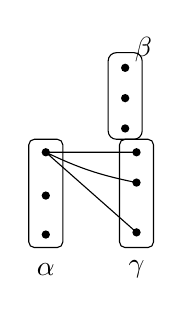
\begin{tikzpicture}[x=0.72cm,y=0.55cm]
\draw[rounded corners=3pt] (1.1,2.5) rectangle (1.7,4.5);
\draw[rounded corners=2pt] (-.3,0) rectangle (.3,2.5);
\draw[rounded corners=2pt] (1.3,0) rectangle (1.9,2.5);
\foreach \x/\y in {1.4/4.15,1.4/3.45,1.4/2.75,0/2.2,0/1.2,0/.3,1.6/2.2,1.6/1.5,1.6/.35}{\fill (\x,\y) circle (1.5pt);}
\draw (0,2.2)--(1.6,2.2) (0,2.2) to[bend right=7] (1.6,1.5) (0,2.2)--(1.6,.35);
\node at (1.72,4.58) {$\beta$};\node at (0,-.5) {$\alpha$};\node at (1.6,-.5) {$\gamma$};
\end{tikzpicture}}

% lower and foot, lines 21–25
à trois éléments associé à $h$, qui n'est autre que $t$ lui-$=$, s'identifie à $I_\gamma$. Les deux trièdres \inserted{$t',t''$} parallèles à $t$ et $\ne t$ sont évidemment celles données par $(j,\beta)$, $j\in I_\alpha\setminus\{i\}$, donc $\varepsilon\simeq I_\alpha-\{i\}$, donc

% foot, last line
\[
h\Leftrightarrow(I_\gamma,I_\alpha\setminus\{i\})
\]

% archive sheet number: 74
\scanpage{76}

% top, lines 1–2
D'autre part $H$ est formé de $t,t',t''$ et des trièdres opposés, donc

% top, lines 3–5
\[
\begin{aligned}
H&\longleftrightarrow(I_\alpha,\{0,1\})\\
&\quad\inserted{\unsure{\text{ou}^{''}|\simeq}\,I_\alpha\setminus\{i\}}\\
\omega(H)&\simeq\omega(I_\alpha)\simeq I_\alpha\setminus\{i\}\\
\omega(h)&\simeq\omega(I_\gamma)
\end{aligned}
\]

% upper, lines 6–7
Il n'y a pas de relation universelle entre ces deux ens à $2$ él\ldots.

% separator and title, lines 8–9
\noindent\rule{1.3cm}{.35pt}\par
\deleted{\unsure{Présent}}\quad\uline{Digression}\quad Présentation symétrique des relations entre \deleted{ens.} \unsure{discrets|objets} de card. $\unsure{2|?},3$ et hexagones.

% middle, line 10
Un hexagone détermine

% middle, a), lines 11–14
a) un ens $\tau$ à trois éléments, qui peut s'interpréter indiff. comme l'ens des diagonales (paires de sommets opposés) ou codiagonales (paires de côtés opposés)

% middle, b), lines 15–17
b) Un ens $\varepsilon$ (de card $2$) \deleted{\unsure{les}} (l'ens des triangles inscrits $=$ triples de sommets biliés)

% middle-lower, b′), lines 18–19
b') Un ens $\varepsilon'$ (de card $2$) l'ens des triangles coinscrits $=$ triples de côtés biliés.

% lower, c), lines 20–23
c) Un iso $\varepsilon\wedge\varepsilon'\overset{\varphi}{\simeq}\omega(\tau)$ (\deleted{\unsure{or. can.}}\inserted{$\simeq$ un ens de gx perm circ. de $\tau$}) \deleted{de $\varepsilon\wedge\varepsilon'$} (i.e iso $\varepsilon'\simeq\omega(\tau)\wedge\varepsilon$. -- $\varepsilon\simeq\varepsilon'\wedge\omega(\tau)$, -- iso $\varepsilon\wedge\varepsilon'\wedge\omega(\tau)=\unsure{1_{\mathbb Z_2}|1_{\mathcal T_2}}$ i.e. un él. de $\varepsilon\wedge\varepsilon'\wedge\omega(\tau)$)

% foot, lines 24–26
On a alors
\[
\begin{aligned}
\text{Sommets}&=\tau\times\varepsilon\\
\text{arêtes}&=\tau\times\varepsilon'
\end{aligned}
\]

% foot, lines 27–28
et rel. d'incidence $(\unsure{s|S},\alpha)$ incident à $(\unsure{t|T},\beta)$ ssi \deleted{\illegible{2}}, $t=\varphi(\alpha\wedge\beta).s$

% archive sheet number: 75
\scanpage{77}

% top, lines 1–3
Le passage d'un hexagone à l'hexagone dual se traduit par le passage de $(\tau,\varepsilon,\varepsilon',\varphi)$ à $(\tau,\varepsilon',\deleted{\unsure{\varepsilon'}}\varepsilon,-\varphi\circ\sigma)$ où $\sigma$ est la symétrie $\varepsilon'\wedge\varepsilon\to\varepsilon\wedge\varepsilon'$.

% upper, line 4
\[
\mathrm{Aut}(h)\subset\mathrm{Aut}(\tau)\times\deleted{\unsure{\mathrm{Aut}\,\varepsilon}}\underbrace{(\pm1)^2}_{\mathrm{Aut}\,\varepsilon\times\mathrm{Aut}\,\varepsilon'}
\]

% upper, line 5
formé des triples $u,\deleted{\unsure{\alpha}}\beta,\deleted{\unsure{\beta}}\gamma$ tels que

% upper, line 6
\[
\deleted{\unsure{\alpha\beta}}\beta\gamma=\mathrm{sg}(\unsure{\tau|u})\qquad\text{ou}\quad\alpha\beta\,\mathrm{sg}(\tau)=1
\]

% upper, lines 7–8
i.e. c'est le sous-gpe de $\mathrm{Aut}\,\tau\times(\pm1)^2$ \unsure{image|formé} inverse de $(\pm1)^{3\prime}=\{(\alpha,\beta,\gamma)\in(\pm1)^3\mid\alpha\beta\gamma=1\}$.

% middle, large diagram
\diagram{\begin{tikzcd}[ampersand replacement=\&,column sep=1.1em,row sep=1.4em,cells={font=\scriptsize}]
|[alias=D]| {\substack{\tau=\text{diagonales}\\\deleted{\unsure{\text{les faces}}}}}\arrow[ddd,"3"'] \& \& |[alias=S]| \text{Sommet}\arrow[ll,"2"']\arrow[ddd,"2"] \&\\
\& |[alias=C]| \text{côtés}\arrow[ul,"2"']\arrow[ddd] \& \&\\
\&[-1em] |[alias=R]| \text{rep. sym.}\arrow[uul,"2"]\arrow[ddd] \& \& |[alias=O]| {\substack{\text{sommets orientés}\\\simeq\text{\unsure{arcs|arêtes|côtés}}\simeq\text{repères}}}\arrow[ul,"2"]\arrow[to=C,"2"]\arrow[ll]\arrow[ddd]\\
|[alias=E]| e \& \& |[alias=B]| {\substack{\varepsilon\\\text{(triangles inscrits)}}}\arrow[ll,"2"'] \&\\
\& |[alias=F]| {\substack{\varepsilon'=\varepsilon\wedge\omega\\\text{\unsure{(triangles circonscr.)|(triangles coinscrits)}}}}\arrow[ul,"2"] \& \&\\
\& |[alias=W]| {\substack{\omega=\omega(\tau)\\\text{orientations}}}\arrow[to=E,"2"'] \& \& {\substack{\varepsilon\times\omega\\\text{triangles}\\\text{inscrits orientés}}}\arrow[ll,"2"]\arrow[to=F,"2"]\arrow[to=B,"2"]
\end{tikzcd}}

% lower, lines 1–3
\uline{NB} Tous les carrés sont cartésiens, y compris les quatre carrés horizontaux de forme triangulaire

% below NB
\diagram{\begin{tikzcd}[ampersand replacement=\&,row sep=small,column sep=small]
{}\&\&{}\arrow[ll]\\
\&{}\arrow[ul]\&\\
\&\&{}\arrow[ul]\arrow[uu]
\end{tikzcd}}

% archive sheet number: 76
\scanpage{78}

% upper left, hexagon and three marks below
\figure{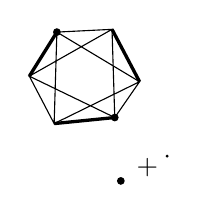
\begin{tikzpicture}[scale=.7]
\coordinate (a) at (-1,0);\coordinate (b) at (-.5,.8);\coordinate (c) at (.5,.85);\coordinate (d) at (1,-.1);\coordinate (e) at (.55,-.75);\coordinate (f) at (-.55,-.86);
\draw (a)--(b)--(c)--(d)--(e)--(f)--cycle (a)--(c)--(e)--cycle (b)--(d)--(f)--cycle;
\draw[very thick] (a)--(b) (c)--(d) (e)--(f);\fill (b) circle (2pt) (e) circle (2pt) (.66,-1.9) circle (2pt);\node at (1.14,-1.65) {$+$};\fill (1.5,-1.45) circle (.8pt);
\end{tikzpicture}}

% top, second sketch
\diagram{\begin{tikzcd}[ampersand replacement=\&,row sep=small,execute at end picture={\draw[thin] ([xshift=-8pt]r.north west) -- ([xshift=-14pt]g.south west);}]
t_1\arrow[r,dash]\arrow[dr,dash]\arrow[ddr,dash]\&|[alias=r]| \alpha\\
t_2\arrow[ur,dash]\arrow[r,dash]\arrow[dr,dash]\&\beta\\
t_0\,{\times}\& |[alias=g]| \gamma
\end{tikzcd}}

% top centre, two short rows
\[
\begin{array}{cccc}
\deleted{\unsure{12|13}}&\unsure{f_{14}}&f_{15}&f_{16}\\
&f_{24}&f_{25}&f_{26}
\end{array}
\]

% top centre, three rows and left arrow
\diagram{\begin{tikzcd}[ampersand replacement=\&,column sep=small,row sep=small]
(t_1,\alpha)\arrow[dr,dash]\arrow[drr,dash]\&(t_1,\beta)\&(t_1,\gamma)\\
(t_2,\alpha)\&(t_2,\beta)\&(t_2,\gamma)\\
(t_0,\alpha)\&(t_0,\beta)\&(\unsure{t_0|t_1},\gamma)\\
{}\&{}\arrow[l]\&
\end{tikzcd}}

% top right, heading and small isolated hexagon
$H$ un hexagone

% top right, by heading
\figure{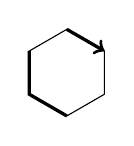
\begin{tikzpicture}[scale=.55]
\draw (90:1)--(30:1)--(-30:1)--(-90:1)--(-150:1)--(150:1)--cycle;
\draw[very thick,->] (90:1)--(30:1);\draw[very thick] (150:1)--(-150:1)--(-90:1);
\end{tikzpicture}}

% upper right, definitions and cardinalities
\[
\begin{aligned}
H_d&\quad\text{ens des diagonales = ens des codiagonales} &&3\\
H_t&\quad\text{ens des triangles inscrits} &&2\\
H_\omega&\quad\text{ens des orientations}\simeq\omega(H_d) &&\big\}2\quad\deleted{\unsure{H_\omega\simeq H_t\wedge\omega(H_d)}}\\
\inserted{H_{t*}}&\quad\inserted{\text{ens des triangles circonscrit}} &&2\\
H_s&\quad\text{ens des sommets}=H_d\times H_t &&6\\
H_{s*}&\quad\text{ens des côtés}=H_d\times H_{t*} &&6\\
H_r&\quad\text{ens des repères}\subset H_s\times H_d &&12\\[-3pt]
&&\text{rel. d'inc. }\text{''}&
\end{aligned}
\]

% under definitions, crossed row and inserted products
\[
\begin{aligned}
&\unsure{H_{r_1}|H_{r'}}\quad H_d\times H_d^{*}\times H_t\times H_{t*}\\
&\deleted{\unsure{H_{s**}|H_{r'}}\quad\text{ens des rep. \unsure{mut.} opp.}=6}\\
&H_{t\mathrm{ror}}=\text{triangles inscrits orientés}\qquad 4
\end{aligned}
\]

% centre and left, network of coverings
\diagram{\resizebox{\linewidth}{!}{\begin{tikzcd}[ampersand replacement=\&,column sep=2.8em,row sep=3.7em,cells={font=\scriptsize}]
\& {\substack{\mathrm{hex}+\mathrm{diag}\\\simeq\mathrm{tria}+\text{él. marqué}\\\simeq\text{couples de trièdres}\\\text{sécants (explicités!)}}}\arrow[d,"3"] \&
{\text{(échanges)}}\arrow[dl,dash]\arrow[d]\&\\
|[alias=A]|{\substack{\mathrm{tria}'=\mathrm{Hex}+\mathrm{diag}\\\mathrm{Hex}+\mathrm{codiag}\\=\text{bib. pliée}}}\arrow[d,"3"] \&
|[alias=B]|{\substack{\mathrm{tria}\simeq\mathrm{hex}\\=\mathrm{Hex}+\text{sommet}}}\arrow[l,"2" description,"\mathrm{opp}"']\arrow[d,"3"] \&
|[alias=C]|{\substack{\mathrm{hexor}\;(\mathrm{hex}+\text{orientation})\\\simeq\mathrm{triaor}\;(\text{trièd.}+\text{ordre circulaire})\\\simeq\omega((\mathrm{hex}+\mathrm{diag})/\mathrm{hex})}}\arrow[l,"2"]\&\\
|[alias=D]|{\deleted{\unsure{\mathrm{H}}}\mathrm{Hex}}\arrow[dd,"3"]\&|[alias=E]|{\substack{\mathrm{trtria}\\\simeq\omega(\mathrm{Hex}/\mathrm{triHex})\ (\mathfrak S_3\text{-tors sur }\mathrm{triHex})\\\simeq\mathrm{Hex}+\text{triangle inscr}\\\simeq\text{pav}+\unsure{\text{coor.}|\text{or.}}}}\arrow[l,"\deleted{\unsure{2}}\,2"']\&{\mathrm{hex}+\text{somm.}}\arrow[l]\arrow[d]\&
{\substack{\mathrm{hex}+\text{triangle inscrit orienté}\\\simeq\text{couples de trièdres orientées}\\\text{parallèles}}}\arrow[ul]\arrow[dl]\\
\&|[alias=F]|{\substack{\mathrm{triaor}'=\mathrm{Hex}\\+\text{rep mod opp}\\(\text{torseur sur }\mathrm{Hex}\\\text{de gpe }\mathfrak S_3)}}\arrow[to=A,"2"]\arrow[d]\arrow[dd,bend left=15,"3"]\&|[alias=G]|{\substack{\deleted{\unsure{\mathrm{Hexrep}}}=\mathrm{Hex}+\mathrm{rep}\simeq\text{couple de trièd. \unsure{liées|fibrées}}\simeq\mathrm{hex}+\text{trièd. marqué}\\\simeq\text{couple de trièdres par.}\\\simeq\mathrm{hex}+\text{``triangle inscr''}\\(\text{torseur sur Hex de gpe }\mathfrak S_3\times\mathfrak S_2)\\\text{torseur sur trtria de gpe }\mathfrak S_3\\\simeq\text{torseur sur triaor gpe }\mathfrak S_2}}\arrow[l,"\mathrm{opp}"']\arrow[to=B,"2"]\arrow[dd]\&\\
{\substack{\deleted{\mathrm{triHex}}\\\mathrm{triHex}}}\&-\mathrm{Pav}\arrow[l,"3"']\&\&\\
\&{\substack{\mathrm{Hexor}\simeq\omega(\mathrm{tria}'/\mathrm{Hex})\\=\mathrm{Hex}+\mathrm{or.}}}\arrow[to=D,"2"]\&
{\substack{\mathrm{trortria}\\\simeq\mathrm{Hex}+\mathrm{tr.or.}\\\text{inscr.}}}\arrow[l,"2"']\arrow[to=E,"2"]\&
\end{tikzcd}}}

% lower right, star and circumscribed sketch
\figure{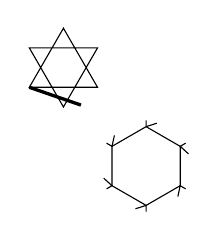
\begin{tikzpicture}[scale=.5]
\draw (90:1)--(210:1)--(330:1)--cycle (150:1)--(270:1)--(30:1)--cycle;\draw[very thick] (210:1)--(-65:1.05);
\begin{scope}[shift={(2.1,-2.5)}]\draw (90:1)--(30:1)--(-30:1)--(-90:1)--(-150:1)--(150:1)--cycle;
\foreach \a in {90,30,-30,-90,-150,150}{\draw (\a:1.16)--(\a:1)--({\a-14}:1.12);}\end{scope}
\end{tikzpicture}}

% bottom middle, list of subgroups
$\mathfrak S_3\times\mathfrak S_2$

$7$ ss-gpes d'indice $2$ \unsure{(3 de ?)|(3 classes)}

$3$ ss-gpes d'indice $4$ (\unsure{conj})

$3$ sous-gpes d'indice $6$ (\inserted{non} conjugués)

% lower right, large marked hexagon over small diagram
\figure{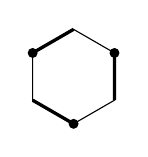
\begin{tikzpicture}[scale=.6]
\draw (90:1)--(30:1)--(-30:1)--(-90:1)--(-150:1)--(150:1)--cycle;
\draw[very thick] (150:1)--(90:1) (30:1)--(-30:1) (-90:1)--(-150:1);
\foreach \a in {150,30,-90}{\fill (\a:1) circle (3pt);}\end{tikzpicture}}

% bottom right, diagram
\diagram{\begin{tikzcd}[ampersand replacement=\&,row sep=small,column sep=small,cells={font=\scriptsize}]
\&H_s\arrow[ddl]\arrow[ddd]\&\&H_r\;\mathfrak S_3\times\mathfrak S_2\arrow[ll]\arrow[dll]\arrow[ddl]\arrow[ddd]\\
\&\mathfrak S_3 H_{r_1}\arrow[dl]\arrow[ddd]\&\&\\
H_d\arrow[ddd]\&\&H_{s*}\arrow[ll]\arrow[ddd]\&\\
\&H_t\arrow[ddl]\&\&H_{t\mathrm{ror}}\arrow[ll]\arrow[dll]\arrow[ddl]\\
\&H_\omega\arrow[dl]\&\&\\
e\&\&H_{t*}\arrow[ll]\&
\end{tikzcd}}

% archive sheet number: 77
\scanpage{79}

% heading
$(\unsure{\mathrm I|+})$ Étude combinatoire des polygones de $3\le n\le6$ côtés

% upper left, sideways note
% margin note written sideways
\margin{On obtient les sous-groupes comme stabilisateurs des sommets (ou côtés) et $\unsure{\sim}$ \unsure{d'un|chacun|chaque} élt de $\unsure{\omega}(T)$\deleted{\illegible{1}}}

% top, 1), lines 2–5
1) \uline{$n=3$}\quad $\mathrm{Pol}_3\simeq(\mathrm{Ens})_3$, le foncteur de dualité est isom can à l'identité (si $P\in\mathrm{Ob}\,\mathrm{Pol}_3$, alors $P^\circ\simeq P$ (iso can.) car les côtés en corr $1-1$ avec les sommets. (Se généralise aux polygônes à un nb impair de côtés. Groupe : $\mathfrak S_{3}$

% upper, 2), lines 6–8
2) \uline{$n=4$}\quad $\mathrm{Pol}_4\xrightarrow{\sim}(\mathrm{Ens})_{2,2}$ (se généralise aux cubes comb. de dim $d\in\mathbb N$, $\mathrm{Cube}_d\simeq(\mathrm{Ens})_{\underbrace{2,2,\ldots,2}_{d}}$) Obtenu en associant à \deleted{\unsure{un C}} carré comb. $C$ l'ens de ses quatre côtés, avec la division en côtés opposés.

% middle, lines 9–15
Le cube combinatoire dim. $2$ est décrit par l'ens des $4$ sommets, avec division en classes de sommets \deleted{\unsure{opposables|opposés}}. Or les sommets correspondent aux sections de $I$ sur $\Lambda$, l'incidence signifiant que les \deleted{côtés} sections ne se rencontrent pas, l'opposition $=$ non incidence signifiant qu'ils sont ``parallèles'' --

% middle left, beside description
\figure{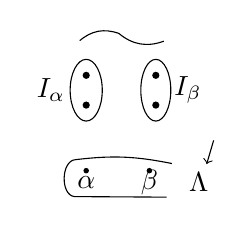
\begin{tikzpicture}[x=.68cm,y=.7cm]
\draw (0,1.1) ellipse (.3 and .56) (1.3,1.1) ellipse (.28 and .56);
\foreach \x in {0,1.3}{\foreach \y in {.83,1.37}{\fill (\x,\y) circle (1.3pt);}}
\node at (-.66,1.1) {$I_\alpha$};\node at (1.9,1.1) {$I_\beta$};
\draw (-.12,2) to[bend left] (.61,2.13) to[bend right] (1.45,1.99);
\draw (1.6,-.23) to[bend right=9] (-.2,-.16) to[bend right=85] (-.22,-.83)--(1.5,-.84);
\node at (0,-.58) {$\alpha$};\node at (1.18,-.58) {$\beta$};\fill (0,-.36) circle (1pt) (1.18,-.36) circle (1pt);
\node at (2.1,-.56) {$\Lambda$};\draw[->] (2.38,.19)--(2.25,-.24);
\end{tikzpicture}}

% lower left, cubical diagram
\diagram{\begin{tikzcd}[ampersand replacement=\&,cells={font=\small},row sep=1.3em,column sep=1.4em]
\& C_s\arrow[dl,"2" description,"\mathrm{opp}"']\& C_r\arrow[l,"2"']\arrow[dl,"2" description,"\mathrm{opp}"']\arrow[dd,"2"]\\
C_d\arrow[dd,"2"']\&C_{r_1}\arrow[l,"2"']\arrow[dl,"2" description]\arrow[dd,"2"]\&\\
C_\omega\arrow[d,"2"']\&\&C_{s*}\arrow[dl,"2" description,"\mathrm{opp}"]\\
e\& C_{d*}\arrow[l,"2"']\&
\end{tikzcd}}
\noindent\unsure{cart}\quad cart\quad cart\quad cart

% lower right, legend
\[
\begin{aligned}
C_r&\quad\text{ens des repères}\\
C_s&\quad\text{------ sommets}\\
C_{s*}&\quad\text{------ côtés}\\
C_d&\quad\text{------ diagonales}=C_s/\mathrm{opp}\\
C_{d*}&\quad\text{------ codiagonales}=C_{s*}/\mathrm{opp}\\
C_{\unsure{\mathrm{op}r|r_1|p'}}&\quad\text{------ repères mod symétrie}\quad C_r/\mathrm{opp}\\
C_\omega&\quad\text{------ orientations}
\end{aligned}
\]

% bottom left, sideways note
% margin note written sideways
\margin{Sauf qu'il y en a $4$ d'ordre $2$ qui se groupent en paires de Sgpes conjugués, engendrés par tr. à $C$ $(\varepsilon.\dot1,\varepsilon.\dot3)$ $(\varepsilon\deleted{\unsure{\dot3}},\varepsilon\dot2)$\ldots}

% bottom, last four lines
$C_r$ est un torseur sous $D_4\simeq\mathfrak S_2\mathbin{.}\mathbb Z/4\mathbb Z$. On trouve que si $r\in C_r$ et si on prend les stabilisateurs des images de ce $r$ dans les ens du diagramme, on trouve exactement $1$ fois et une seule chaque sous-groupe de $D_4$ ! (il y en a exactement $8$, y compris $e$ et $D_4$

% archive sheet number: 78
\scanpage{80}

% top, lines 1–3
\[
\begin{aligned}
3)\quad n=6,\qquad &\mathbb P_6\simeq\mathbb P_3\times(\mathrm{Ens})_2\\
&\text{(marche chaque fois qu'on a $\mathbb P_n$ avec $n=2m$, $m$ impair\ldots)}\\
\text{d'où}\qquad &\mathbb P_6\simeq(\mathrm{Ens})_3\times(\mathrm{Ens})_2
\end{aligned}
\]

% upper, lines 4–7
Si $t\in(\mathrm{Ens})_{\deleted{\unsure{2}}3}$ et $\omega\in(\mathrm{Ens})_2$, \deleted{le polyg} l'hexagone associé a comme sommets les él. de $t\times\omega$, et $(a,\alpha)$ $(b,\beta)$ \deleted{\unsure{adjts}} liés sss $a\ne b$, $\alpha\ne\beta$ : \uline{L'hexagone est une bitriade}.

% upper-middle, lines 7–11
Ici, pour un hexagone donné $H$, \inserted{si $\mathrm{opp}$ est la symétrie antipodique} il y a bijection canonique entre l'ens $H_s/\mathrm{opp}\simeq\deleted{\unsure{H_t}}H_d$ des diag. et l'ens $H_{d*}$ des \deleted{\unsure{côtés}} codiag. (paires de côtés opposés) en associant à ch. diagonale la paire des $2$ côtés parallèles à celle-ci.

% middle, below paragraph
\[\boxed{H_d\simeq H_{d*}}\quad(=t)\]

% middle, lines 12–14
Soit $H_{\mathrm{tr}}$ l'ens des \inserted{$2$} ``triangles inscrits'' -- c'est $\varepsilon$\deleted{\unsure{\xi}} bien sûr, \inserted{-- ou l'ens des trièdres constituant l'hexagone --} $H_{\mathrm{tr}*}$ l'ens des triangles circonscrits

% above diagram
On a maintenant le diagramme

% left of diagram
\figure{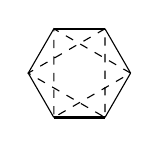
\begin{tikzpicture}[scale=.65]
\foreach \a in {0,60,120,180,240,300}{\draw (\a:1)--({\a+60}:1);}
\draw[dashed] (0:1)--(120:1)--(240:1)--cycle (60:1)--(180:1)--(300:1)--cycle;
\draw[thick] (60:1)--(120:1) (240:1)--(300:1);
\end{tikzpicture}}

% middle-lower, diagram
\diagram{\begin{tikzcd}[ampersand replacement=\&,row sep=1em,column sep=1.5em,cells={font=\scriptsize}]
\& H_s\arrow[ddl,"2" description,"\mathrm{opp}"']\arrow[ddd,"3"]\&\&H_r\,D_6\arrow[ll,"2"']\arrow[dll,"2" description,"\mathrm{opp}"']\arrow[ddl,"2"]\arrow[ddd,"3"]\\
\&H_{r'}\,\mathfrak S_3\arrow[dl,"2"]\arrow[ddd]\&\&\\
H_d\arrow[ddd,"3"']\&\&H_{s*}\arrow[ll,"2" description,"\mathrm{opp}"]\arrow[ddd,"3"]\&\\
\&H_{\mathrm{tr}}\arrow[ddl,"2"']\&\&H_{\mathrm{tror}}\,\mathbb F_2^2\arrow[ll,"2"']\arrow[dll,"2"]\arrow[ddl,"2"]\\
\&H_\omega\arrow[dl,"2"']\&\&\\
e\&\&H_{\mathrm{tr}*}\arrow[ll,"2"']\&
\end{tikzcd}}

% right of diagram
\margin{\uline{NB} tous les carrés cart. toutes les fl. hor. de degré $2$ \rule{2em}{.3pt} vert \rule{2em}{.3pt} $3$}

% below diagram, four braced notes
\[
\mathrm{Nb}\ \left\{\begin{aligned}
H_d&=\text{ens des sommets d'un triangle inscrit ou circonscrit}\\
H_\omega&=\text{ens des orientations de }H\simeq\omega(H_d)\simeq H_{\mathrm{tr}}\wedge H_{\mathrm{tr}*}\\
H_{r'}&=H_r/\mathrm{opp}\simeq\text{ens des rep. de }H_d\text{ (donc $\mathfrak S_3$-torseur)}\\
H_{\mathrm{tr}}\times H_{\mathrm{tr}*}&\simeq H_{\mathrm{tr}}\times H_\omega\simeq H_{\mathrm{tror}}\quad\text{ens des 4 triangles \unsure{inscrit|inscrits} \uline{orientés}}
\end{aligned}\right.
\]

% foot, lines 1–6
Ceci correspond au diagramme des sous groupes de
\[
D_6=\mathfrak S_2\mathbin{.}\mathbb Z/6\mathbb Z\simeq\mathfrak S_2\times\mathfrak S_3\quad\text{d'ordre }12.\quad D_6.
\]
ayant \inserted{trois} \deleted{\unsure{un}} sous-groupes \inserted{(conjugués)} d'indice $3$ (stabilisateurs des \inserted{trois} él. de $H_d$) $3$ sous-groupes \inserted{(deux à deux \inserted{non} conjugués)} d'indices $2$ (stabilisateurs des él. de $H_{\mathrm{tr}},H_{\mathrm{tr}*},H_\omega$ respectivement), un sous-gpe d'indice $4$ (stabilisateur des él. de $H_{\mathrm{tror}}$)

% archive sheet number: 79
\scanpage{81}

% upper, lines 1–8
enfin trois \deleted{familles} \inserted{classes de conjugaison} de ss-gpes \deleted{conjugués} d'indice $6$, \inserted{i.e. d'ordre $2$} comprenant un gpe invariant (i.e. formant une seule classe), savoir le centre, qui est le stabilisateur des él. de $H_{r'}$, et $2$ \deleted{familles} \inserted{classes} de \inserted{$3$ ss-}groupes chacunes \deleted{\unsure{comprenant}} resp. stabilisateurs des él. de $H_s$ et $H_{s*}$ : les \deleted{\unsure{$\varepsilon$}} $u$ \inserted{et les $zu$} ($z$ él. non triv. du centre, i.e. gén. du facteur $\mathbb Z/2\mathbb Z=\mathfrak S_2$ de $\mathfrak S_2\times\mathfrak S_3$, $u$ el. d'ordre $2$ de $\mathfrak S_3$) \deleted{et} \deleted{\unsure{les $zu$}}

% middle, lines 9–15
Les classes de conj. de ss-gpes de $D_6$ correspondent encore \inserted{$1-1$} aux \deleted{classes} espaces hom. du diagramme marqué, et on constate que les autom. de ces espaces homogènes sont ceux marqués sur le diagramme (une flèche $\xrightarrow{2}$ i.e. d'ordre $3$ impliquant qu'il y a à la source un autom. inv. (ss pt fixe) --).

% archive sheet number: 80
\scanpage{82}

% heading, lines 1–2
Carrés et hexagones dans un pavé

$X$ pavé.

% upper, I), lines 3–6
I) L'ens des carrés $C\subset X$ est en corr $1-1$ avec l'ens (des sommets de) $X$, à tout carré $C$ correspondant l'unique $x\in X$ non lié \deleted{aux sommets} \inserted{à tous les sommets} de $C$, \inserted{et à $a\in C$ l'ens des pts de $C$ non liés à \unsure{$a$}} (\uline{NB} il y a un seul pt de $X$ \inserted{non} lié à \deleted{deux pt} deux pts distincts

% left of upper paragraph
\figure{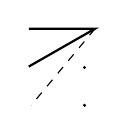
\begin{tikzpicture}[scale=.6]
\draw[thick] (0,1.1)--(1.4,1.1)--(0,.3);\draw[dashed] (1.4,1.1)--(.05,-.52);\fill (1.18,.28) circle (1pt) (1.18,-.52) circle (1pt);
\end{tikzpicture}}

% upper-middle, lines 7–11
non liés -- i.e. \unsure{tte|à} \deleted{\unsure{couple|angle}} \inserted{paire} de pts \deleted{distincts} non liés est contenue dans un trièdre unique -- la donnée d'un tel couple équivaut \inserted{donc} à la donnée d'un trièdre pointée $(t,a)$, en associant à $(t,a)$ la paire $t\setminus\{a\}$ ]

% middle, lines 11–17
Pour que $2$ paires de pts non liés $\{x,x'\}$ $\{y,y'\}$ forment un carré, il faut s. que \deleted{les trièdres} leur ``centre'' $a$ soit le \unsure{$\overline{=}$|$\overline{\mathrm m}$}, i.e qu'elles sont disjointes et \deleted{appartiennent} à deux trièdres \uline{sécants} ; la donnée d'une \deleted{diagonale} des paires $\{x,x'\}$ détermine alors l'autre sans ambiguité ; $\{y,y'\}$ est aussi l'ens des pts de $X$ liés à ceux de $\{x,x'\}$.

% middle left, next to pairs
\diagram{\begin{tikzcd}[ampersand replacement=\&,column sep=tiny,row sep=tiny]
y\arrow[rr,dash]\arrow[dd,dash]\&\&x'\arrow[dd,dash]\\
\&\cdot\&\\
x\arrow[rr,dash]\&\&y'
\end{tikzcd}}

% middle right margin
\figure{\begin{tikzpicture}[x=.16cm,y=.13cm]
\foreach \x/\y in {0/0,1/0,2/0,0/1,1/1,2/1,0/2,1/2,2/2}{\fill[black!55] (\x,\y) circle (.5pt);}
\end{tikzpicture}}

% lower, lines 18–22
Donc la donnée d'un carré à diagonale marquée équivaut à celle d'une paire de pts non liés, ou encore à celle d'une trièdre pointée.

La donnée d'un carré à sommet marqué équivaut à celle d'une trièdre épinglée !

% lower left, three clusters
\figure{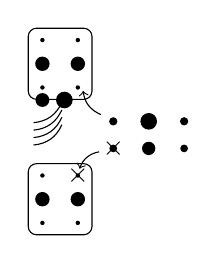
\begin{tikzpicture}[x=.45cm,y=.43cm]
\foreach \off in {0,4}{\draw[rounded corners=3pt] (-.4,\off-.35) rectangle (1.4,\off+1.75);
\foreach \x in {0,1}{\foreach \y in {0,.7,1.4}{\fill (\x,\off+\y) circle (.8pt);}\fill (\x,\off+.7) circle (2.6pt);}}
\node at (1,1.4) {$\times$};
\foreach \x in {2,3,4}{\fill (\x,3) circle (1.5pt);\fill (\x,2.2) circle (1.4pt);}\fill (3,3) circle (3pt) (3,2.2) circle (2.4pt);\node at (2,2.2) {$\times$};\fill (0,3.63) circle (2.5pt) (.62,3.63) circle (3pt);
\draw[->] (1.65,3.2) to[bend left] (1.15,3.9);\draw[->] (1.6,2.1) to[bend right] (1.05,1.6);
\foreach \j in {0,.22,.44,.66}{\draw[thin] (-.25,2.3+\j) to[bend right] (.55,2.9+\j);}
\end{tikzpicture}}

% lower, lines 23–24
\[
\begin{aligned}
\deleted{\unsure{\mathrm{Car}_d}}\quad\mathrm{Car}_d(X)&\simeq\mathrm{triapt}(X)\\
\mathrm{Car}_s(X)&\simeq\mathrm{tria\,ép}(X)\quad\text{(est un $\mathfrak S_3$-ens libre!)}
\end{aligned}
\]

% foot, lines 25–26
\deleted{\unsure{tres|Les autres}} \inserted{Chacun des $4$} pts de $X\setminus C$ distinct du centre $a$ de $C$ est donc lié à exactement un point de la diag $\{x,x'\}$, et

% archive sheet number: 81
\scanpage{83}

% top to middle, lines 1–10
de $\overline{=}$ pour l'autre diagonale $\{y,y'\}$, donc $Y=X\setminus(C\cup\{a\})$ s'envoie dans le produit des diagonales et on trouve là une bijection. Ces $4$ pts sont d'ailleurs liés à $a$, ce sont les $4$ sommets des deux triangles de sommet $a$. On voit donc aussi que l'ombre sur $C$ d'un pt de $Y$ est un côté de $C$, et qu'on trouve une corr. $1-1$ de $C$ avec l'ens des \inserted{$4$} côtés de $C$. \deleted{Deux} Deux pts de $Y$ sont liés sss \deleted{$\mathrm{Car}_{s*}(C)\unsure{\simeq}$} \deleted{leur} ils correspondent à des côtés opposés de $C$.

% middle, lines 11–12
Donc les $2$ paires de côtés opposés de $C$ correspondent aux $2$ triangles de sommet $a$.

% middle left, by first display
\figure{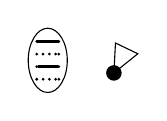
\begin{tikzpicture}[x=.4cm,y=.4cm]
\draw (0,0) ellipse (.62 and 1.02);
\foreach \y in {-.6,-.2,.2,.6}{\foreach \x in {-.35,-.15,.05,.25,.35}{\fill (\x,\y) circle (.55pt);}}
\draw[very thick] (-.35,.6)--(.35,.6) (-.32,-.2)--(.33,-.2);
\draw (2.1,-.4)--(2.15,.55)--(2.86,.21)--cycle;\fill (2.1,-.4) circle (2.8pt);
\end{tikzpicture}}

% middle, lines 13–14
Donc
\[
\begin{aligned}
\mathrm{Car}_{d*}(X)&\simeq\mathrm{trgpt}(X)\\
\mathrm{Car}_{s*}(X)&\simeq\mathrm{arc}(X)\simeq\deleted{\unsure{\mathrm{arctr}}}\mathrm{trgép}(X)\quad\text{(c'est un $\mathfrak S_3$-ens libre!)}
\end{aligned}
\]

% middle left, by second equivalence
\figure{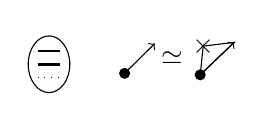
\begin{tikzpicture}[x=.48cm,y=.48cm]
\draw (0,0) ellipse (.55 and .75);\draw[thick] (-.3,.36)--(.3,.36);\draw[very thick] (-.3,0)--(.3,0);\draw[dotted] (-.3,-.36)--(.3,-.36);
\fill (2,-.24) circle (2pt);\draw[->] (2,-.24)--(2.8,.55);\node at (3.25,.17) {$\simeq$};\draw (4,-.28)--(4.08,.48)--(4.9,.58)--cycle;\draw[->] (4,-.28)--(4.9,.58);\node at (4.08,.48) {$\times$};\fill (4,-.28) circle (2pt);
\end{tikzpicture}}

% lower middle, lines 15–17
d'où
\[
C_{r'}(X)\simeq\text{ens des couples d'un trièdre et d'un triangle sécants dans $X$}
\]

% left, by Cr′
\figure{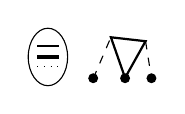
\begin{tikzpicture}[x=.5cm,y=.5cm]
\draw (0,0) ellipse (.5 and .73);\draw[thick] (-.27,.27)--(.27,.27);\draw[very thick] (-.27,0)--(.27,0);\draw[dotted] (-.27,-.25)--(.27,-.25);
\draw[thick] (1.6,.5)--(2.48,.4)--(1.96,-.53)--cycle;\draw[dashed] (1.15,-.55)--(1.6,.5) (2.48,.4)--(2.63,-.54);\foreach \x in {1.15,1.96,2.63}{\fill (\x,-.54) circle (1.8pt);}
\end{tikzpicture}}

% lower, lines 18–19
Enfin
\[
C_r(X)\simeq\text{épinglages du pavé}
\]

% lower left, by Enfin
\figure{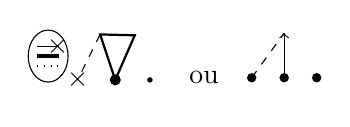
\begin{tikzpicture}[x=.55cm,y=.55cm]
\draw (0,0) ellipse (.46 and .6);\draw (-.25,.23)--(.25,.23);\node at (.22,.23){$\times$};\draw[very thick] (-.25,0)--(.25,0);\draw[dotted] (-.25,-.23)--(.25,-.23);
\draw[thick] (1.2,.5)--(2,.48)--(1.55,-.55)--cycle;\draw[dashed] (1.2,.5)--(.68,-.55);\node at (.68,-.55){$\times$};\fill (1.55,-.55) circle (2pt) (2.35,-.55) circle (1pt);
\node at (3.6,-.5) {ou};\draw[dashed] (4.7,-.5)--(5.45,.53);\draw[->] (5.45,-.5)--(5.45,.53);\foreach \x in {4.7,5.45,6.2}{\fill (\x,-.5) circle (1.7pt);}
\end{tikzpicture}}

% right margin, sideways covering diagram
% margin note written sideways
\diagram{\begin{tikzcd}[ampersand replacement=\&,column sep=large,row sep=large,cells={font=\scriptsize}]
{\substack{\mathrm{Hex}_d\\(\simeq\mathrm{tria}'\simeq\mathrm{pav}+\mathrm{ab})}}\arrow[d,"3"']\&{\substack{\mathrm{Hex}_s\simeq\mathrm{hex}\\\simeq\mathrm{tria}}}\arrow[l,"2"']\arrow[d,"3"]\&\\
{\substack{\mathrm{Hex}\\(\simeq\mathrm{pav})}}\arrow[d,"3"']\&{\substack{\mathrm{Hex}_{\mathrm{tr}}\\(\simeq\mathrm{pavcoor})\\\simeq\mathrm{trtria}}}\arrow[l,"2"']\&\\
\mathrm{triHex}\&\mathrm{Hex}_{s*}\arrow[uul,"2"]\arrow[d,"3"]\&\mathrm{Hex}_{\text{ép}}\arrow[l,dash,"\unsure{2}"']\arrow[uul,"2"]\arrow[d,"3"]\\
\&{\substack{\mathrm{Hex}_{\mathrm{tr}*}\\\text{(triples de bases}\\\text{en position particulière)}}}\arrow[uul,"2"]\&\mathrm{Hex}_{\mathrm{tror}}\arrow[l,"2"']\arrow[uul,"2"]
\end{tikzcd}}

% foot, left scribbled sketch
\figure{
\begin{tikzpicture}[scale=.48]
\foreach \x in {0,.45,.9}{\foreach \y in {0,.51,1.02}{\fill (\x,\y) circle (1.2pt);}}
\fill (0,1.02) circle (2.5pt);\node at (.65,1.02) {$\times$};
\foreach \k in {0,.25,.5,.75}{\draw (-.13,\k)--(.7,{\k+.5})--(.03,\k);}
\end{tikzpicture}}

% foot, lines 20–22
\unsure{et|alors}\quad $C_\omega(X)=\unsure{C_{r'}(X)}/\mathrm{opp}$ \deleted{\unsure{au lieu}} \inserted{$\mathrm{opp}=$} passage d'un couple d'un trièdre et triangle sécants, au couple opposé.

% archive sheet number: 82
\scanpage{84}

% top, lines 1–2
exactement -- ceci correspond à $4$ carrés de $\overline{=}$ centre $a$).

% upper, question
\uline{Question} Quels sont les graphes finis qui ont \unsure{aussi|ainsi} une ``enveloppe'' \inserted{pseudo} \unsure{trialitaire|trilatère} ? Exemples.

% upper left, rounded outline beside examples
\figure{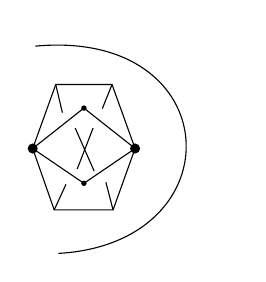
\begin{tikzpicture}[scale=.65]
\draw (-.55,1.25)--(.55,1.25)--(1,0)--(.57,-1.2)--(-.58,-1.2)--(-1,0)--cycle;
\draw (-1,0)--(0,.79)--(1,0)--(0,-.68)--cycle (-.55,1.25)--(-.42,.7) (.55,1.25)--(.36,.78) (-.58,-1.2)--(-.35,-.7) (.57,-1.2)--(.43,-.66);
\draw (-.17,.4)--(.2,-.44) (.18,.4)--(-.13,-.4);\fill (-1,0) circle (2.8pt) (1,0) circle (2.8pt) (0,.79) circle (1.5pt) (0,-.68) circle (1.5pt);
\draw (-.95,2) .. controls (2.8,2.35) and (3,-1.85) .. (-.5,-2.05);
\end{tikzpicture}}

% upper middle, six examples
\diagram{\begin{tikzcd}[ampersand replacement=\&,row sep=1.2em,column sep=.9em,cells={font=\scriptsize}]
\bullet\arrow[d]\&\rule{1.3em}{1.5pt}\arrow[d]\&
\tikz[baseline=-.6ex]{\draw (0,0) rectangle (.5,.48);\draw[very thick] (0,0)--(.5,0);}\arrow[d]\&
\tikz[baseline=-.6ex]{\draw (90:.3)--(18:.3)--(-54:.3)--(-126:.3)--(162:.3)--cycle;\draw[very thick] (-54:.3)--(-126:.3);}\arrow[d]\&
\tikz[baseline=-.6ex]{\draw (100:.3)--(30:.3)--(-38:.3)--(-114:.3)--(168:.3)--cycle;\draw[very thick] (100:.3)--(30:.3)--(-38:.3)--(-114:.3);}\arrow[d]\&
\tikz[baseline=-.6ex]{\draw[very thick] (-.2,.3)--(.2,.3) (-.2,-.2)--(.2,-.2);\draw[thin,rounded corners=3pt] (-.34,-.25)--(-.42,.12)--(-.25,.48)--(.32,.47)--(.42,.16)--(.29,-.27)--(.14,-.38)--cycle;}\arrow[d]\\
\bullet\&\unsure{\text{arête}}\&\text{pavé}\&\text{pavé}\&\unsure{\text{carré}}\&
\tikz[baseline=-.6ex]{\draw (-.14,0)--(.17,.46)--(-.03,.46)--(.12,0)--cycle;}
\end{tikzcd}}

% upper right and below examples
(et bien sûr les complexes \inserted{pseudo} trialitaires eux-$\overline{=}$s) et les \deleted{de graphes} graphes intermédiaires entre ceux-ci et leur enveloppe

% above middle examples
Regarder p.ex. \unsure{les}

% middle, upper row of examples
\figure{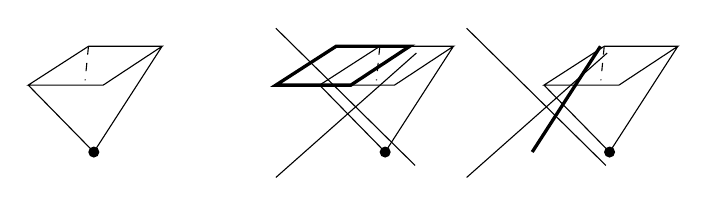
\begin{tikzpicture}[x=.85cm,y=.85cm]
\foreach \k in {0,3.7,6.55}{\begin{scope}[xshift=\k cm]
\draw (0,0)--(.9,.58)--(2,.58)--(1.12,0)--cycle (0,0)--(.98,-1)--(2,.58);\draw[dashed] (.9,.58)--(.85,.07);\fill (.98,-1) circle (2pt);\end{scope}}
\draw[very thick] (3.7,0)--(4.6,.58)--(5.7,.58)--(4.82,0)--cycle (7.53,-1)--(8.55,.58);
\foreach \k in {3.7,6.55}{\draw (\k,.85)--({\k+2.08},-1.2) (\k,-1.38)--({\k+2.1},.48);}
\end{tikzpicture}}

% middle left, below Regarder
\deleted{\unsure{graphes}} \deleted{Regarder}

% middle, lower row of examples
\figure{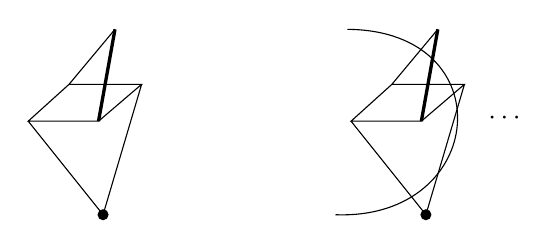
\begin{tikzpicture}[x=.72cm,y=.72cm]
\foreach \k in {0,4.1}{\begin{scope}[xshift=\k cm]\draw (0,0)--(.72,.65)--(2,.65)--(1.24,0)--cycle (0,0)--(1.32,-1.65)--(2,.65) (.72,.65)--(1.53,1.62);\draw[very thick] (1.53,1.62)--(1.24,0);\fill (1.32,-1.65) circle (2pt);\end{scope}}
\draw (5.63,1.62) .. controls (8.4,1.6) and (8.1,-1.75) .. (5.42,-1.65);
\node at (8.4,.05) {$\cdots$};
\end{tikzpicture}}

% across middle
\noindent\rule{\linewidth}{.35pt}

% lower right, three shape labels
\figure{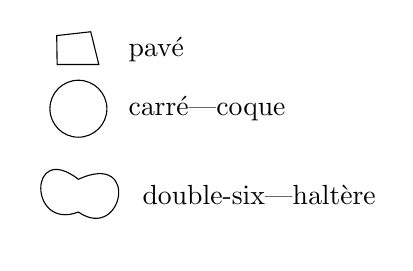
\begin{tikzpicture}[scale=.54]
\draw (-.5,0)--(.48,0)--(.29,.77)--(-.51,.68)--cycle;\node[right] at (.95,.36) {pavé};
\draw (0,-1.04) circle (.67);\node[right] at (.95,-1.04) {\unsure{carré|coque}};
\draw (0,-2.7) .. controls (-1.18,-1.78) and (-1.18,-3.92) .. (0,-3.47) .. controls (1.04,-4.19) and (1.47,-2.02) .. (0,-2.7);\node[right] at (1.28,-3.07) {\unsure{double-six|haltère}};
\end{tikzpicture}}

% lower field, covering diagram and adjacent point clusters
\diagram{\begin{tikzcd}[ampersand replacement=\&,column sep=2em,row sep=2.2em,cells={font=\scriptsize}]
{\times\ \bullet\ \cdot}\& {\substack{\mathrm{Car}_s\simeq\mathrm{hex}_s\\\unsure{\updownarrow|\wr}\\\mathrm{tria}\,\text{ép}}}\arrow[r]\arrow[dl,dash]\&{\substack{\mathrm{Car}_{\mathrm{rep}}\\\unsure{\updownarrow|\wr}\\\mathrm{hex}\,\text{ép}}}\arrow[dl,dash]\arrow[d,bend left=18]\arrow[dll]\\
{\substack{\mathrm{Car}_d\sim\mathrm{hex}_d\\\unsure{\updownarrow|\wr}\simeq\deleted{\unsure{\mathrm{Hex}}}_d\\\mathrm{tria}\,\mathrm{pt}}}\arrow[d,dash]\&
{\substack{\mathrm{Car}_{r'}\simeq\mathrm{hex}_{s*}}}\arrow[l]\arrow[d]\&
{\unsure{\mathrm{Car}_{s*}}}\arrow[dl,dash]\\
{\substack{\mathrm{Car}\\\simeq\mathrm{pav}\,\mathrm{pt}}}\arrow[r,dash]\&\mathrm{Car}_{d*}\&
\end{tikzcd}}

% lower field, miniature figures surrounding diagram
\figure{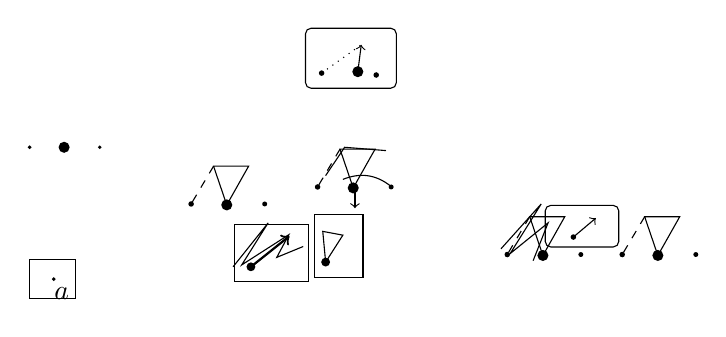
\begin{tikzpicture}[x=.73cm,y=.6cm]
\foreach \x/\r in {0/.7, .6/2,1.22/.7}{\fill (\x,2) circle (\r pt);}
\draw[rounded corners=2pt] (4.8,3.25) rectangle (6.38,4.52);\fill (5.08,3.57) circle (1pt) (5.71,3.6) circle (2pt) (6.03,3.53) circle (1pt);\draw[->] (5.71,3.6)--(5.77,4.17);\draw[dotted] (5.08,3.57)--(5.77,4.17);
\foreach \x/\y in {3.2/1.6,5.4/1.96,8.7/.53,10.7/.53}{\begin{scope}[shift={(\x,\y)}]\draw (0,0)--(.23,-.82)--(.61,0)--cycle;\draw[dashed] (0,0)--(-.39,-.8);\fill (.23,-.82) circle (2pt) (-.39,-.8) circle (1pt) (.89,-.8) circle (.9pt);\end{scope}}
\draw[->] (5.66,1.13)--(5.66,.71);\draw (5.15,1.4)--(5.48,2)--(6.2,1.93);\draw (5.45,1.32) to[bend left] (6.28,1.18);
\draw[rounded corners=2pt] (8.97,-.11) rectangle (10.25,.77);\draw[->] (9.46,.1)--(9.85,.5);\fill (9.46,.1) circle (1pt);
\draw[thin] (8.2,-.15)--(8.9,.8)--(8.36,-.25)--(9.02,.4)--(8.76,-.4);
\draw (0,-1.2) rectangle (.8,-.38);\fill (.42,-.79) circle (.7pt);\node at (.56,-1.1){$a$};
\draw (3.56,-.84) rectangle (4.85,.36) (4.95,-.76) rectangle (5.8,.57);
\fill (3.85,-.53) circle (1.6pt) (5.15,-.43) circle (1.6pt);\draw[->,thick] (3.85,-.53)--(4.52,.12);\draw (5.15,-.43)--(5.45,.14)--(5.1,.22)--cycle;
\draw[thin] (3.54,-.53)--(4.15,.4)--(3.69,-.49)--(4.51,.15)--(4.3,-.33)--(4.76,-.1);
\end{tikzpicture}}

% foot right, four labels
\diagram{\begin{tikzcd}[ampersand replacement=\&,row sep=small]
{\text{\uuline{$\mathrm{Car}$}}_d}\arrow[r,dash]\arrow[d,phantom,"\unsure{\wr\!\vert|\wr}"]\&{\text{\uuline{$\mathrm{Car}$}}}\arrow[dr]\\
\mathrm{hex}_d\arrow[r,dash]\&\mathrm{hex}\&{}
\end{tikzcd}}

% archive sheet number: 83
\scanpage{85}

% top, two lines of cancelled opening
\uline{NB} \deleted{La correspondance $C\longmapsto X\setminus\{C\cup\{\unsure{a|\cdot}\}\}$ entre carrés de $X$ et}

% upper and middle, lines 2–9
Appelons \uline{anticarré} l'opposé d'un carré, i.e. un graphe somme de deux segments. Les anticarrés dans $X$ sont donc les carrés dans $X^\circ$, qui est un pavé, donc ils correspondent aux pts de $X^\circ$, en associant à \unsure{tt|$\forall$} $a\in X^\circ$ l'ens des $4$ pts de $X^\circ$ qui sont $X^\circ$-\unsure{non}liés à $a$, i.e. qui sont $X$-liés à $a$. \deleted{Interpréter les} Donc

% middle, lines 10–15
la correspondance $C\longmapsto(X\setminus C\cup\{a=\text{centre de }C\}\unsure{\}})$ entre carrés de $X$ et anticarrés de $X$ est bijective. Si $C$ et $C'$ sont associés ainsi, $C$ et $C'^\circ$ sont des carrés en dualité (les sommets de l'un étant les côtés de l'autre.

% lower, lines 16–22
Il y a une corr. fonctorielle évidente qui associe à chaque carré $C$ un pavé \inserted{$\mathrm{Pav}(C)$} le contenant (son ``enveloppe'') dont l'ens des sommets est $C\amalg C^{*\circ}\amalg\{a\}_{\text{centre}}$. Deux points de $C$ ($C^{*\circ}$) sont liés ssi ils sont liés dans $C$ (\deleted{\unsure{non}}\inserted{resp} liés dans $C^{*\circ}$ i.e non liés dans $C^*$), un pt \inserted{$x$} de $C$ est lié à un pt \inserted{$x^{*}$} de $C^{*\circ}$ ssi \deleted{\unsure{sont}} $x,x^*$ incidents, enfin $a$ est non lié aux pts de $C$, lié aux

% archive sheet number: 84
\scanpage{86}

% top, lines 1–4
de $C^{*\circ}$. L'opposé de ce pavé \inserted{$\mathrm{Pav}(C)^\circ$} est can. isom \deleted{au pavé} \inserted{à} $\mathrm{Pav}(C^*)$, \deleted{\unsure{mais}} \unsure{Obtenu|Obtenir}, en \deleted{\unsure{notant que}} \deleted{\unsure{transformant de l'autre côté}}, \inserted{utilisant l'iso.} $\deleted{\unsure{\text{can}}}C^{**}\simeq C$ -- qui est l'isom can. composé avec l'antipodisme\ldots

% upper, display and annotations
\[
\mathrm{Pav}(\underset{\substack{\diagup\\\text{carré}\\\text{donné}}}{C})^\circ
\overset{\text{canon}}{\simeq}
\mathrm{Pav}(\underset{\substack{\diagup\\\text{carré dual de }C}}{C^*})
\]

% middle, NB
\uline{NB} Le produit des deux symétries de $X$ relatives aux triangles issus de $a$ est celui qui \deleted{échange entre eux les} \inserted{fixe $a$ et} induit l'antipodisme sur $C$ et sur $C^{*\circ}$

% middle-lower, universal property
$C\hookrightarrow\mathrm{Pav}(C)$ a la propriété universelle évidente pour les complexes trialitaires $\unsure{\mathcal X|\mathscr X}$ :

% lower, first display
\[
\mathrm{Pl}(\mathrm{Pav}(C),\mathcal X)\xrightarrow{\sim}\mathrm{Pl}(C,X)\qquad\text{(plongts)}
\]

% lower, next line
Si $\mathcal X$ est lui-$\overline{=}$ un pavé, on écrit

% lower, second display
\[
\mathrm{Iso}(\mathrm{Pav}(C),\mathcal X)\simeq\mathrm{Pl}(C,\mathcal X)
\]

% lower, final implication
Pour $\mathcal X$ complexe trialitaire donné, \deleted{\unsure{une}} la donnée d'un carré dans $\mathcal X$ revient à la donnée d'un \uline{pavé pointé} (car un carré est contenu dans un pavé unique\ldots)

% foot, NB and inline figure
\uline{NB} On fera attention que dans un graphe cubique un \uline{anticarré} (s'insérant \unsure{un.} dans un bitriangle
\figure{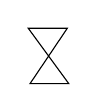
\begin{tikzpicture}[scale=.46]\draw (-.55,.77)--(.53,.77)--(-.5,-.76)--(.57,-.76)--cycle;\end{tikzpicture}}
) est contenu dans \uline{4} pavés

% archive sheet number: 85
\scanpage{87}

% top, heading and first formula
graphe produit de graphes $(\Gamma_i)\ (i\in I)$

% top, vertex set
\[
\text{ens des sommets}\qquad\prod\Gamma_i
\]

% top, adjacency and addition
$x=(x_i)$ et $y=(y_i)$ \deleted{distincts} liés ssi $\exists\,i\in I$ tel que $x_j=y_j$ si $j\ne i$, et $x_i,y_i$ liés
\inserted{c'est op. associative (pas produit catégorique.)}

% upper, opposite graph
graphe \deleted{\unsure{opposé}} $\Gamma^\circ$ \deleted{\unsure{dual}} opposé du graphe $\Gamma$ : $=$ sommets, deux pts \inserted{distincts} de $\Gamma^\circ$ sont liés ssi ils sont non liés dans $\Gamma$.

% upper middle, NB
NB pour un $\Gamma$ donné, l'ens des structures de \deleted{\unsure{la}} graphes \inserted{(strict)} \deleted{\unsure{correspond en bijection par dualité avec l'ens des structures de}} \inserted{$=$} l'ens des parties de \inserted{$^{\wedge}$} $\mathfrak P_2(\Gamma)$, \unsure{la|le} \deleted{\unsure{dualité}} \inserted{opposition} est le passage au complémentaire. C'est une involution qui, pour $\mathfrak P_2(\Gamma)\ne\varnothing$ i.e. $\mathrm{card}(\Gamma)\ge 2$, est sans pt fixe. Néanmoins, il peut arriver que $\Gamma$ soit isomorphe au graphe \deleted{dual}. On dit alors que $\Gamma$ est ``\uline{auto\deleted{dual}\inserted{opposé}}''.

% middle, coproduct definition
\uline{coproduit} de graphes $\Gamma_i$ : \inserted{graphe $\Gamma=\overset{\circ}{\prod}\Gamma_i$} défini par $\Gamma^\circ=\prod_i\Gamma_i^\circ$ \inserted{(notation $\Gamma_1\mathbin{\overset{\circ}{\times}}\Gamma_2$ pour deux facteurs,}
\deleted{$\unsure{\Gamma=}$}
\[
\Gamma=\left(\prod_i\Gamma_i^\circ\right)^\circ\quad\text{i.e.}
\]

% middle-lower, vertices and condition
Donc ens des sommets de $\Gamma$ \deleted{\unsure{est}} $=\prod_i\Gamma_i$. Deux sommets $x=(x_i)$ et $y=(y_i)$ \inserted{de $\Gamma$} sont \inserted{\uline{non}} liés (dans $\Gamma$) ssi ils sont \deleted{non} liés dans $\Gamma^\circ$, i.e. ssi $\exists\,i\in I$ tel que $x_j=y_j$ pour $j\ne i$, et $x_i,y_i$ \deleted{\unsure{non}} liés dans $\Gamma_i^\circ$, i.e. $x_i,y_i$ \uline{non} liés dans $\Gamma_i$. On a prouvé la

% left of condition
\margin{\uline{NB} $\left(\prod\Gamma_i\right)^\circ=\overset{\circ}{\prod}\Gamma_i^\circ$ \deleted{\unsure{donc}}.}

% lower, proposition
\uline{Prop} Un pavé (i.e. \inserted{graphe iso. au} produit de deux triangles) est autodual, en d'autres termes un pavé est isomorphe au coproduit de deux trièdres (duals des triangles) ou encore un coproduit de deux trièdres est un pavé.

% archive sheet number: 86
\scanpage{88}

% top, coproduct
Coproduit \inserted{d'un graphe} avec un doublet $\bullet\quad\bullet$ donne, pour un graphe discret, les \unsure{bigraphes|graphes} bidiscrets.

% upper, doublets
Coproduit de deux doublets $(\underset a\bullet\ \underset b\bullet)\ (\underset{a'}\bullet\ \underset{b'}\bullet)$

% upper, crossed pairs
\diagram{\begin{tikzcd}[ampersand replacement=\&,row sep=small,column sep=small]
(ba')\arrow[dr,dash] \& (bb')\arrow[dl,dash]\\
(aa') \& (ab')
\end{tikzcd}}

% upper middle, segments
\unsure{Coproduit|produit} de deux segments $(\underset{a}{\bullet}\!-\!\underset{b}{\bullet})\quad(\underset{a'}{\bullet}\!-\!\underset{b'}{\bullet})$

% upper middle, square 1
\diagram{\textcircled{1}\quad\begin{tikzcd}[ampersand replacement=\&,row sep=small,column sep=small]
(ba')\arrow[r,dash]\arrow[d,dash]\arrow[dr,dash,draw=gray] \& (bb')\arrow[d,dash]\arrow[dl,dash,draw=gray]\\
(aa')\arrow[r,dash] \& (ab')
\arrow[from=1-1,to=2-2,phantom,"\deleted{\times}"]
\end{tikzcd}\qquad carré}

% middle, opposite and bracketed passage
\deleted{\unsure{dual}} opposé du précédent. [Le \uline{produit} de \deleted{\unsure{un doublet} $\underset{a}{\bullet}\ \underset b\bullet$ et d'un segment $\underset{a'}\bullet\!-\!\underset{b'}\bullet$} \inserted{deux doublets est l'ens à quatre él. discret} \deleted{\unsure{alors par}} le coproduit de deux segments est donc le graphe chaotique à $4$ él. -- ces deux \unsure{résultats|doublets|semble} \unsure{peu|purs} \unsure{enthousiasmants|contrairement|intéressants}\ldots]

% middle below fold
Produit d'un doublet \inserted{$(a\bullet\ \bullet b)$} et d'un segment \inserted{$a'\bullet\!-\!\bullet b'$}

% lower middle, two horizontal segments
\diagram{\begin{tikzcd}[ampersand replacement=\&,row sep=small,column sep=small]
(ba')\arrow[r,dash] \& (bb')\\ (aa')\arrow[r,dash] \& (ab')
\end{tikzcd},}

% lower, opposite
son opposé est le coproduit du segment $(\overset a\bullet\!-\!\overset b\bullet)$ et du doublet $(a'\bullet\ \bullet b')$

% lower, square 2
\diagram{\textcircled{2}\quad\begin{tikzcd}[ampersand replacement=\&,row sep=small,column sep=small]
(ba')\arrow[d,dash]\arrow[dr,dash] \& (bb')\arrow[d,dash]\arrow[dl,dash,crossing over]\\
(aa') \& (ab')
\end{tikzcd}\qquad\uline{carré}}

% foot, continuation
Donc sur le produit de deux ens de cardinal $2$, on trouve $3$ structures de carré naturelles distinctes, \deleted{\unsure{comme}} savoir la structure \uline{produit} de deux \uline{segments}

% archive sheet number: 87
